\documentclass{standalone}
\usepackage{tikz}
\usetikzlibrary{patterns, positioning}

\begin{document}
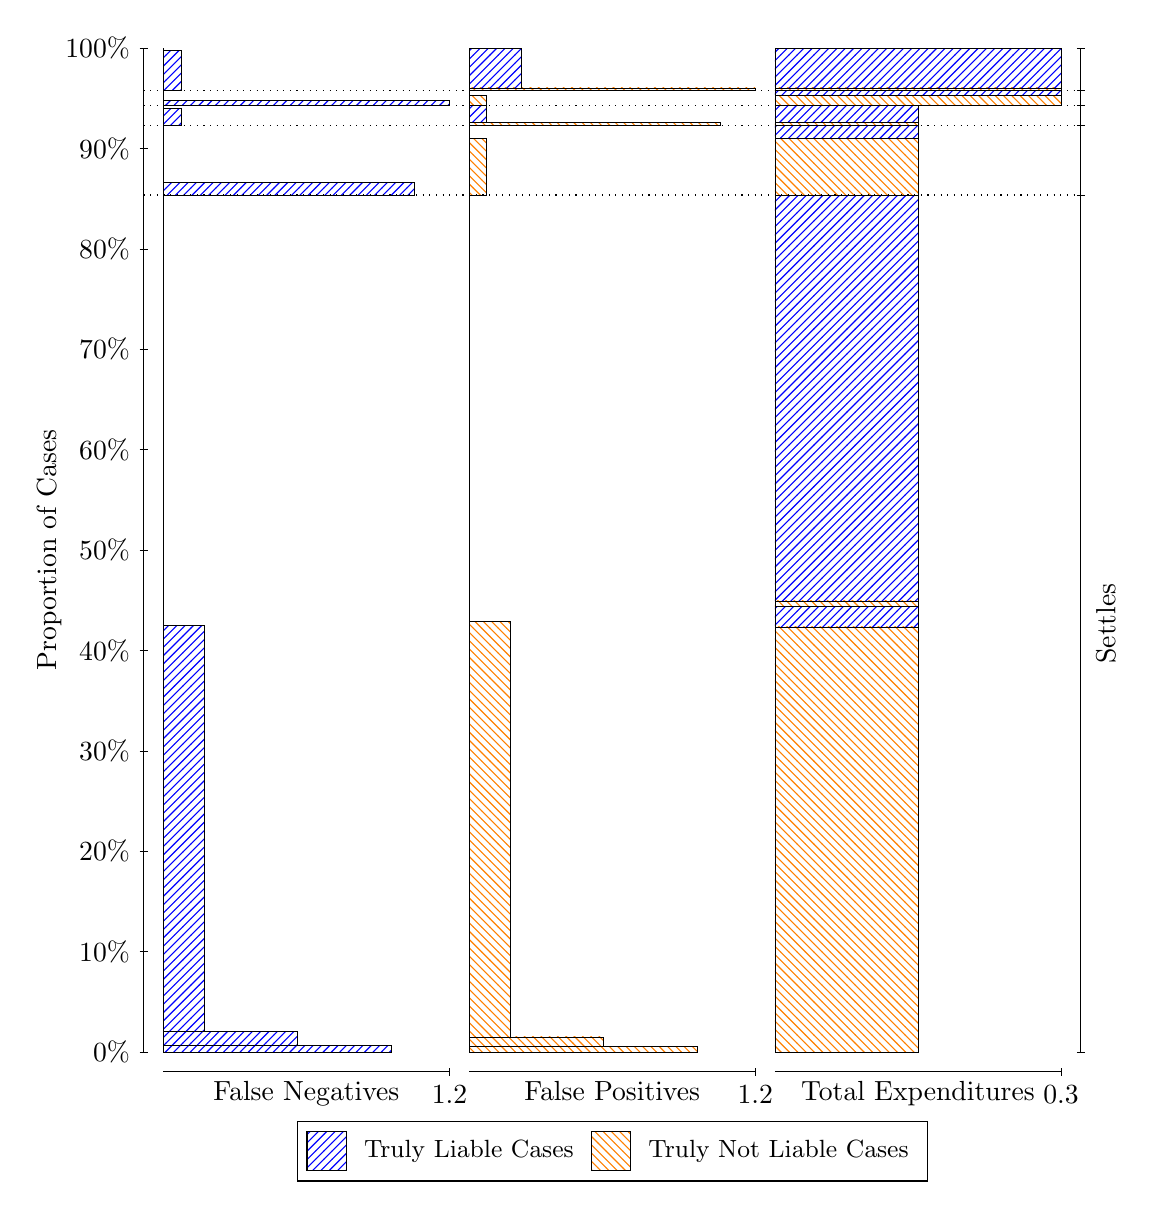
\begin{tikzpicture}
\draw[black, very thin] (1.5,1.75) -- (1.5,14.5);
\node[rotate=90, anchor=center] at (0.3, 8.125) {Proportion of Cases};
\draw[black, very thin] (1.45,1.75) -- (1.55,1.75);
\node[anchor=east] at (1.45, 1.75) {0\%};
\draw[black, very thin] (1.45,3.025) -- (1.55,3.025);
\node[anchor=east] at (1.45, 3.025) {10\%};
\draw[black, very thin] (1.45,4.3) -- (1.55,4.3);
\node[anchor=east] at (1.45, 4.3) {20\%};
\draw[black, very thin] (1.45,5.575) -- (1.55,5.575);
\node[anchor=east] at (1.45, 5.575) {30\%};
\draw[black, very thin] (1.45,6.85) -- (1.55,6.85);
\node[anchor=east] at (1.45, 6.85) {40\%};
\draw[black, very thin] (1.45,8.125) -- (1.55,8.125);
\node[anchor=east] at (1.45, 8.125) {50\%};
\draw[black, very thin] (1.45,9.4) -- (1.55,9.4);
\node[anchor=east] at (1.45, 9.4) {60\%};
\draw[black, very thin] (1.45,10.675) -- (1.55,10.675);
\node[anchor=east] at (1.45, 10.675) {70\%};
\draw[black, very thin] (1.45,11.95) -- (1.55,11.95);
\node[anchor=east] at (1.45, 11.95) {80\%};
\draw[black, very thin] (1.45,13.225) -- (1.55,13.225);
\node[anchor=east] at (1.45, 13.225) {90\%};
\draw[black, very thin] (1.45,14.5) -- (1.55,14.5);
\node[anchor=east] at (1.45, 14.5) {100\%};

\draw[black, very thin] (13.4,1.75) -- (13.4,14.5);
\draw[black, very thin] (13.35,1.75) -- (13.45,1.75);
\node[anchor=west] at (13.35, 1.75) {};
\draw[black, very thin] (13.35,12.633) -- (13.45,12.633);
\node[anchor=west] at (13.35, 12.633) {};
\draw[black, very thin] (13.35,13.515) -- (13.45,13.515);
\node[anchor=west] at (13.35, 13.515) {};
\draw[black, very thin] (13.35,13.775) -- (13.45,13.775);
\node[anchor=west] at (13.35, 13.775) {};
\draw[black, very thin] (13.35,13.965) -- (13.45,13.965);
\node[anchor=west] at (13.35, 13.965) {};
\draw[black, very thin] (13.35,14.5) -- (13.45,14.5);
\node[anchor=west] at (13.35, 14.5) {};

\draw[black, very thin, pattern color=blue, pattern=north east lines] (1.75,1.75) rectangle (4.6418,1.8374);
\draw[black, very thin, pattern color=blue, pattern=north east lines] (1.75,1.8374) rectangle (3.4554,2.0128);
\draw[black, very thin, pattern color=blue, pattern=north east lines] (1.75,2.0128) rectangle (2.269,7.1667);
\draw[black, very thin, pattern color=orange, pattern=north west lines] (1.75,7.1667) rectangle (1.75,12.633);
\draw[black, very thin, pattern color=blue, pattern=north east lines] (1.75,12.633) rectangle (4.9384,12.798);
\draw[black, very thin, pattern color=orange, pattern=north west lines] (1.75,12.798) rectangle (1.75,13.515);
\draw[black, very thin, pattern color=blue, pattern=north east lines] (1.75,13.515) rectangle (1.9724,13.738);
\draw[black, very thin, pattern color=orange, pattern=north west lines] (1.75,13.738) rectangle (1.75,13.775);
\draw[black, very thin, pattern color=blue, pattern=north east lines] (1.75,13.775) rectangle (5.3833,13.839);
\draw[black, very thin, pattern color=orange, pattern=north west lines] (1.75,13.839) rectangle (1.75,13.965);
\draw[black, very thin, pattern color=blue, pattern=north east lines] (1.75,13.965) rectangle (1.9724,14.471);
\draw[black, very thin, pattern color=orange, pattern=north west lines] (1.75,14.471) rectangle (1.75,14.5);
\draw[black, very thin, pattern color=orange, pattern=north west lines] (5.6333,1.75) rectangle (8.5252,1.8166);
\draw[black, very thin, pattern color=orange, pattern=north west lines] (5.6333,1.8166) rectangle (7.3388,1.9426);
\draw[black, very thin, pattern color=orange, pattern=north west lines] (5.6333,1.9426) rectangle (6.1524,7.2161);
\draw[black, very thin, pattern color=blue, pattern=north east lines] (5.6333,7.2161) rectangle (5.6333,12.633);
\draw[black, very thin, pattern color=orange, pattern=north west lines] (5.6333,12.633) rectangle (5.8558,13.349);
\draw[black, very thin, pattern color=blue, pattern=north east lines] (5.6333,13.349) rectangle (5.6333,13.515);
\draw[black, very thin, pattern color=orange, pattern=north west lines] (5.6333,13.515) rectangle (8.8218,13.552);
\draw[black, very thin, pattern color=blue, pattern=north east lines] (5.6333,13.552) rectangle (5.8558,13.775);
\draw[black, very thin, pattern color=orange, pattern=north west lines] (5.6333,13.775) rectangle (5.8558,13.901);
\draw[black, very thin, pattern color=blue, pattern=north east lines] (5.6333,13.901) rectangle (5.6333,13.965);
\draw[black, very thin, pattern color=orange, pattern=north west lines] (5.6333,13.965) rectangle (9.2667,13.994);
\draw[black, very thin, pattern color=blue, pattern=north east lines] (5.6333,13.994) rectangle (6.3007,14.5);
\draw[black, very thin, pattern color=orange, pattern=north west lines] (9.5167,1.75) rectangle (11.333,7.1495);
\draw[black, very thin, pattern color=blue, pattern=north east lines] (9.5167,7.1495) rectangle (11.333,7.4123);
\draw[black, very thin, pattern color=orange, pattern=north west lines] (9.5167,7.4123) rectangle (11.333,7.4789);
\draw[black, very thin, pattern color=blue, pattern=north east lines] (9.5167,7.4789) rectangle (11.333,12.633);
\draw[black, very thin, pattern color=orange, pattern=north west lines] (9.5167,12.633) rectangle (11.333,13.349);
\draw[black, very thin, pattern color=blue, pattern=north east lines] (9.5167,13.349) rectangle (11.333,13.515);
\draw[black, very thin, pattern color=orange, pattern=north west lines] (9.5167,13.515) rectangle (11.333,13.552);
\draw[black, very thin, pattern color=blue, pattern=north east lines] (9.5167,13.552) rectangle (11.333,13.775);
\draw[black, very thin, pattern color=orange, pattern=north west lines] (9.5167,13.775) rectangle (13.15,13.901);
\draw[black, very thin, pattern color=blue, pattern=north east lines] (9.5167,13.901) rectangle (13.15,13.965);
\draw[black, very thin, pattern color=orange, pattern=north west lines] (9.5167,13.965) rectangle (13.15,13.994);
\draw[black, very thin, pattern color=blue, pattern=north east lines] (9.5167,13.994) rectangle (13.15,14.5);
\draw[black, dotted] (1.5,12.633) -- (13.4,12.633);
\draw[black, dotted] (1.5,13.515) -- (13.4,13.515);
\draw[black, dotted] (1.5,13.775) -- (13.4,13.775);
\draw[black, dotted] (1.5,13.965) -- (13.4,13.965);
\draw[black, very thin] (1.75,1.5) -- (5.3833,1.5);
\node[anchor=north] at (3.5667, 1.5) {False Negatives};
\draw[black, very thin] (5.3833,1.45) -- (5.3833,1.55);
\node[anchor=north] at (5.3833, 1.45) {1.2};

\draw[black, very thin] (5.6333,1.5) -- (9.2667,1.5);
\node[anchor=north] at (7.45, 1.5) {False Positives};
\draw[black, very thin] (9.2667,1.45) -- (9.2667,1.55);
\node[anchor=north] at (9.2667, 1.45) {1.2};

\draw[black, very thin] (9.5167,1.5) -- (13.15,1.5);
\node[anchor=north] at (11.333, 1.5) {Total Expenditures};
\draw[black, very thin] (13.15,1.45) -- (13.15,1.55);
\node[anchor=north] at (13.15, 1.45) {0.3};

\node[black, centered, rotate=90] at (13.72, 7.1914) {Settles};





\draw (7.449999999999999,1.5) node[draw=none] (baseCoordinate) {};
\begin{scope}[align=center]
        \matrix[scale=0.5, draw=black, below=0.5cm of baseCoordinate, nodes={draw}, column sep=0.1cm]{
            \node[rectangle, draw, minimum width=0.5cm, minimum height=0.5cm, pattern=north east lines, pattern color=blue] {}; &
            \node[draw=none, font=\small] (B) {Truly Liable Cases}; &
            \node[rectangle, draw, minimum width=0.5cm, minimum height=0.5cm, pattern=north west lines, pattern color=orange] {}; &
            \node[draw=none, font=\small] (B) {Truly Not Liable Cases}; \\
            };
\end{scope}

\end{tikzpicture}
\end{document}